\section{Проектирование ИС}

	При проектировании новой ИС в перую очередь было уделено внимание тому, что разрабатываемая система может использоваться не только в связке с платформой дистанционного обучения, но и как самостоятельная ИС. По этому реализуемая система включает в себя две части: независимая ИС для проверки на плагиат и надстройка в виде плагина для платформы дистанционного обучения.

	Кодовое название ИС: <<Шерлок>>.

	Работа с ИС <<Шерлок>> предпологает два варианта: синхронный и асинхронный. В первом варианте при запросе на проверку клиент будет ожидать результата проверки всё время обработки запроса, а во втором варианте клиенту после первого запроса вернётся ункальный идетификатор проверяемой работы, по которому он в дальшейшем сможет получить результат проверки. В случае, если при проверке работы сотрудником учебного заведения работа ещё не прошла проверку на плагиат, то сотрудник может вручную запустить процесс проверки работы. 

	Интеграция платформы дистанционного обучения Moodle с ИС <<Шерлок>> происходит с помощью плагина, основная задача которого - это регулярная проверка наличия новых работ в системе <<Moodle>> и отправка таких работ на проверку в ИС <<Шерлок>>, а так же отображение результата проверки.

	\subsection{Cистема управления базами данных}

		В качестве СУБД в проекте была выбрана документо-ориентированая база <<MongoDB>> по следующим причинам:
		\begin{itemize}
			\item гибкая модель данных, отличная от той, что предлагают реляционные БД. В ИС <<Шерлок>> модель данных представляет из себя очень ограниченный набор типов объектов и их взаимоотношений между собой, и по этой причне нет необходимости в реляционной алгебре, которая является основой работы традиционных СУБД;
			\item простая установка и настройка. Даже когда появиится потребность в распределённой БД, добавление новых узлов не потребует много усилий;
			\item тестная интеграция с уже существующими технологиями.
		\end{itemize}

	\subsection{Технологии, используемые для реализации ИС}

		В связи с разделением проекта на две части, ИС <<Шерлок>> (``backend'') и плагин для платформы дистанционного обучения (``frontend''), в проекте представлено два технологических стека.

		\subsubsection{ИС <<Шерлок>>}

			В качестве программной платформы для реализации ИС <<Шерлок>> была выбрана платформа ``Java'' по следующим причинам:
			\begin{itemize}
				\item платформа ``Java'' является платформонезависимой, то есть система, написаная на этой платформе может запускаться на огромном числе различных ОС без каких-либо изменений в исходных кодах системы;
				\item за долгое время развития этой платформы было создано огромное число различных готовых инструментов для решения самых различных задач.
			\end{itemize}

			Основной паттерн взаимодействия с ИС - это принятие запроса, его обработка и отправка ответа. Предпологается, что взаимодействие с ИС может происходить из разных сторонних систем, которые могут быть реализованы на совершенно различных технологических стеках. В связи с этим, протокол взаимодействия должет быть таким, который доступен в как можно большем числе технологий. В качестве такого метода взаимодействия был выбран принцип взаимодействия REST на основе протокола HTTP, так как протокол HTTP имеет широкое распространение в Интернете и для работы с ним уже существует большое число готовых решений.

			Для разработки ИС на платформе ``Java'' существует ряд фреймворков, в которых уже реализована часть типовых задач, с которыми чаще всего сталкиваются разработчики. В качестве таких задач могут выступать работа с различными сетевыми протоколами, управление безопастностью приложения, валидация данных, работа с хранилищами данных, поддержка механизма внедрения зависимостей и другие задачи. В данном проекте в качестве такого фреймворка был выбран Spring Framework по ряду причин:
			\begin{itemize}
				\item активная разработка и поддержка этого фреймворка даёт возможность легко использовать многие современные технологии, используемые при разработке ПО;
				\item за долгую историю развития (более 10 лет) вокруг этого фреймворка сформировалось большое сообщество разработчиков и было написано большое число литературы;
				\item данный фреймворк построен по принципу модульности, что позволяет использовать только те части, которые действительно требуются в проекте.
			\end{itemize}

		\subsubsection{Плагин для платформы дистанционного обучения}

			Расширение функционала для ИС <<Moodle>> осуществляется с помощью плагинов, которые описываются на языке программиирования PHP \cite{Moore2010}. 

	\subsection{Сравнение аналогов}

		На данный момент для решения вопроса автоматизации проверки работ на плагиат уже существует ряд систем, наиболее распространённые из которых описываются ниже (JPlag, MOSS).

		JPlag - это система, которая позволяет определять схожесть исходных кодов, написанных на языках Java, C, C++, C\# и Scheme. Так же имеется возможность проверки обычных текстовых документов. Данный сервис доступен как веб-сервис. В качестве алгоритма сравнения работ JPlag использует алгоритм <<greedy string tiling>> \cite{Wise1993}. При использовании этого алгоритма его сложность в худшем случае - $O(n^3)$, а в лучшем - $O(n^2)$ \cite{Prechelt2002}.  Для повышения эффективности работы алгоритма проверки применяется алгоритм Рабина — Карпа \cite{Burrows2007} \cite{Karp1987}, с которым сложность становится почти линейной - $O(n^{1,12})$. Результат сравнения представляется в виде HTML-страницы, на которой отображаются заимствованные части проверяемой работы.

		MOSS (Measure Of Software Similarity) - система проверки на плагиат, доступная как веб-сервис. Имеется возможность проверки работ на таких языках программирования, как Java, C, C++, Scheme. В качестве методов для сверки работ используются <<fingerprinting technique>> и алгоритм <<Winnowing>> \cite{Winnowing2003}.		

		В ходе анализа уже существующих решений был определён ряд требований, которыми в совокупности не обладает ни одна из рассмотренных систем:
		\begin{itemize}
			\item независимость от третьих лиц и возможность установки системы в рамках университета, для полного контроля над нею;
			\item возможность проверки различных типов текстовых документов;
			\item расширяемость функционала - возможность определения алгоритмов, которые используются для проверки и добавление новых типов проверяемых работ (разные языки программирования);
			\item простота использования для конечного пользователя - сотрудника учебного заведения.
		\end{itemize}

	\subsection{Визуальное проектирование ИС}

		Для лучшего понимания тех или иных аспектов в работе и структуре ИС был разработан ряд диаграмм с использованием нотации UML \cite{Fowler2003}.

		\subsubsection{Диаграмма прецедентов}

			Для определения круга задач, решаемых с помощью разрабатываемой системой с точки зрения пользователя, была разработана диаграмма прецедентов (рис. \ref{img:use_case_diagram}), на которой отображены основные пользователи, взаимодействующие с системой, а также возможности, доступные для них.
			\newline
			\newline
			\begin{figure}[h]
				\center{\frame{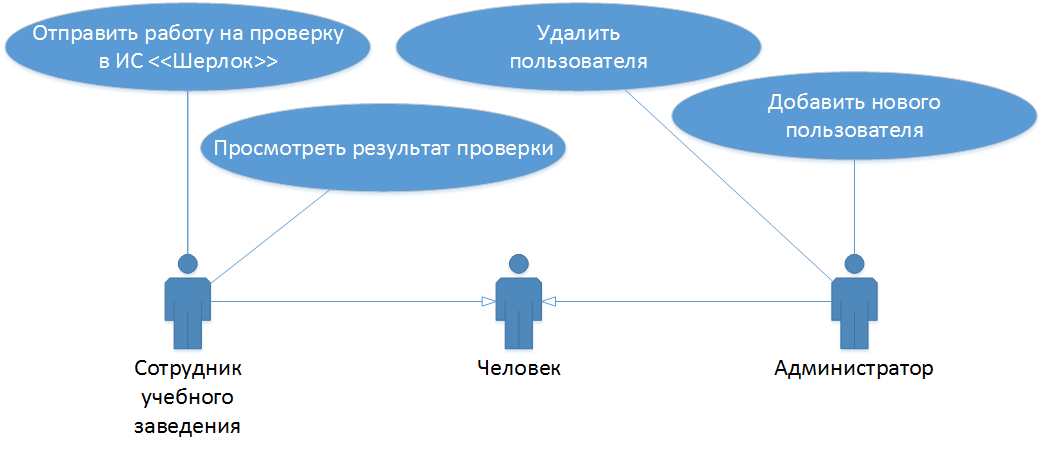
\includegraphics[width=0.8\linewidth]{use_case_diagram.png}}}
				\caption{Диаграмма прецедентов}
				\label{img:use_case_diagram}
			\end{figure}
			
			Описание прецедентов:
			\begin{itemize}
				\item ``Отправить работу на проверку в ИС <<Шерлок>>'' \\
				Предусловие: нахождение на странице проверяемой работы. \\
				Действующее лицо: сотрудник учебного заведения. \\
				Основной поток: отправка работы на проверку на плагиат. \\
				Альтернативный поток: в ходе проверки возникла ошибка. Необходима ручная проверка. \\
				Описание: сотрудник отправляет работу на проверку в ИС <<Шерлок>> на выявление факта плагиата. \\
				Постусловие: работа отправлена на проверку. \\

				\item ``Просмотереть результаты проверки'' \\
				Предусловие: нахождение на странице работы, для которой был получен результат проверки. \\
				Действующее лицо: сотрудник учебного заведения. \\
				Основной поток: просмотр результата проверки. \\
				Альтернативный поток: результат проверки не представлен. Необходима ручная проверка. \\
				Описание: сотрудник просматривает результаты проверки работы на плагиат, для которой он отправлял запрос. \\
				Постусловие: сотрудник просмоетрел результат. \\

				\item ``Добавить нового пользователя'' \\				
				Действующее лицо: администратор. \\
				Основной поток: добавление новго пользователя в ИС <<Шерлок>>. \\
				Альтернативный поток: новый пользователь не добавлен. Попробывать ещё раз с новыми данными о пользователе. \\
				Описание: администратор добавляет нового пользователя в ИС <<Шерлок>>, что бы тот смог отправлять работы на проверку и просматривать результаты проверки. \\
				Постусловие: в ИС <<Шерлок>> добавлен новый пользователь. \\

				\item ``Удалить пользователя'' \\				
				Действующее лицо: администратор. \\
				Основной поток: удаление пользователя из ИС <<Шерлок>>. \\
				Альтернативный поток: удаление не выполнено. Попробывать ещё раз с новыми данными о пользователе. \\
				Описание: администратор пользователя из ИС <<Шерлок>>. \\
				Постусловие: пользователь удалён из ИС <<Шерлок>>.
			\end{itemize}

		\subsubsection{Диаграмма классов}

			Для описания модели объектов и их взаимодействия между собой была составлена диаграмма классов (рис. \ref{img:class_diagram}).
			\newline
			\begin{figure}[h]
				\center{\frame{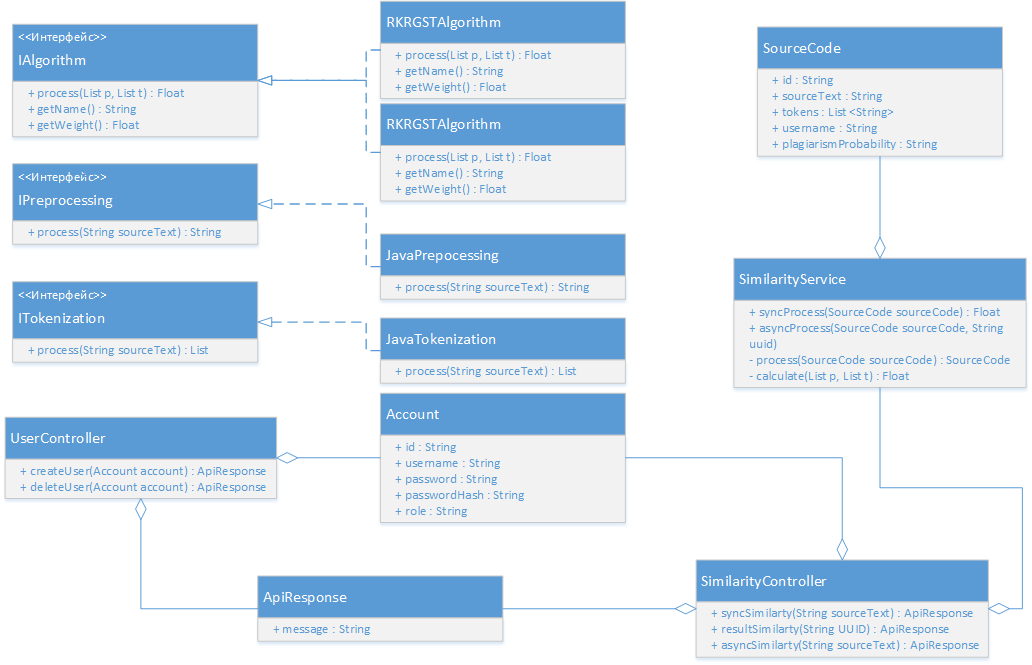
\includegraphics[width=0.9\linewidth]{class_diagram.png}}}
				\caption{Диаграмма классов}
				\label{img:class_diagram}
			\end{figure}

		\newpage
		\subsubsection{Диаграмма последовательности}

			На рис. \ref{img:sequence_diagram} представлена диаграмма последовательности, которая описывает наиболее частый сценарий использования ИС - обработка синхронного запроса на проверку работы.	
			\newline
			\begin{figure}[h]
				\center{\frame{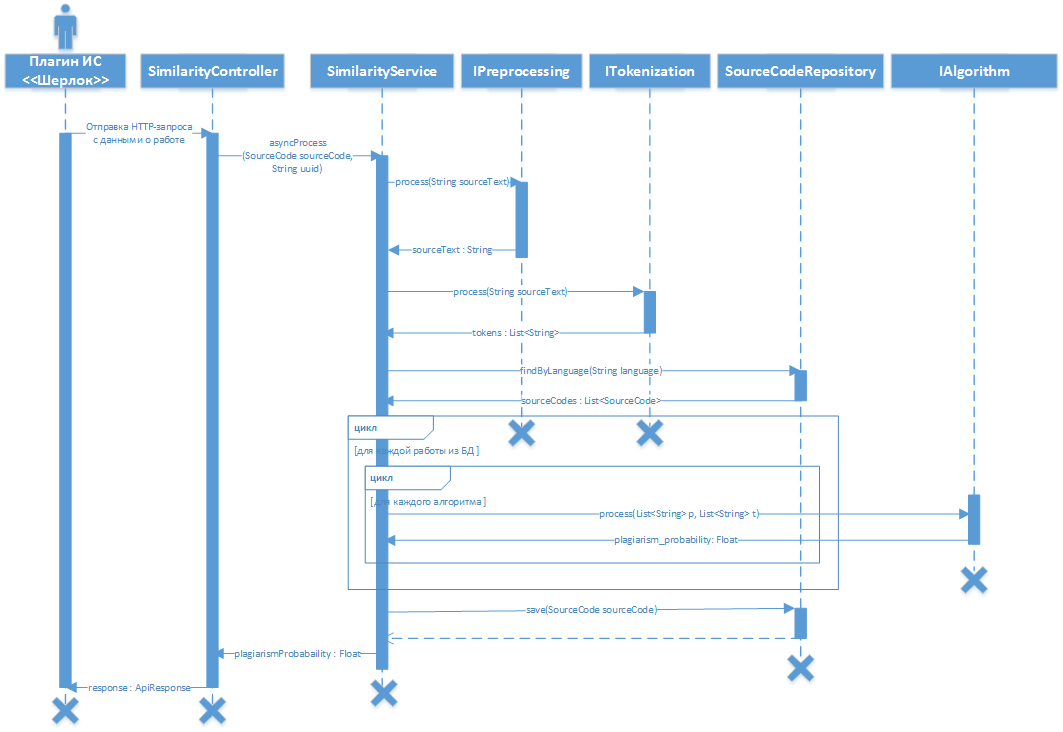
\includegraphics[width=0.95\linewidth]{sequence_diagram.png}}}
				\caption{Диаграмма последовательности}
				\label{img:sequence_diagram}
			\end{figure}

		\newpage
		\subsubsection{Диаграмма развёртывания}

			На рис. \ref{img:deployment_diagram} представлена диаграмма развёртывания, на которой отображено взаимодействие между разными компонентами ИС.
			\newline
			\begin{figure}[h]
				\center{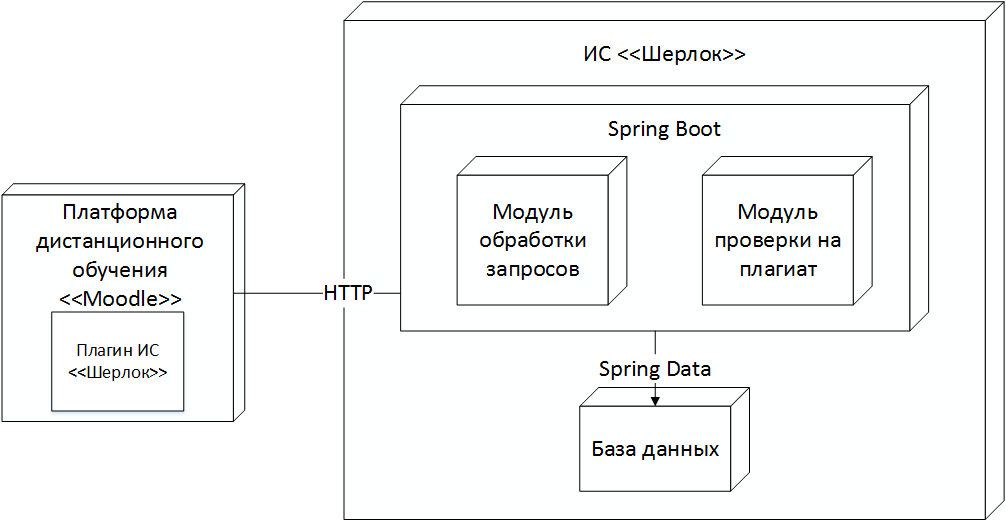
\includegraphics[width=0.95\linewidth]{deployment_diagram.png}}
				\caption{Диаграмма последовательности}
				\label{img:deployment_diagram}
			\end{figure}